\documentclass[10pt,twocolumn]{article}

% ── Packages ──────────────────────────────────────────────────────────────────
\usepackage[a4paper, top=2cm, bottom=2cm, left=1.8cm, right=1.8cm,
            columnsep=0.6cm]{geometry}
\usepackage{times}
\usepackage{amsmath,amssymb}
\usepackage{graphicx}
\usepackage{xcolor}
\usepackage{booktabs}
\usepackage{array}
\usepackage{tabularx}
\usepackage{multirow}
\usepackage{enumitem}
\usepackage{hyperref}
\usepackage{fancyhdr}
\usepackage{titlesec}
\usepackage{caption}
\usepackage{subcaption}
\usepackage{tikz}
\usepackage{pgfplots}
\pgfplotsset{compat=1.18}
\usetikzlibrary{shapes.geometric, arrows.meta, positioning, fit, backgrounds, calc}
\usepackage{float}
\usepackage{microtype}
\usepackage{setspace}
\usepackage{abstract}

% ── Color definitions ─────────────────────────────────────────────────────────
\definecolor{darkblue}{HTML}{1a237e}
\definecolor{medblue}{HTML}{1565c0}
\definecolor{lightblue}{HTML}{e3f2fd}
\definecolor{accent}{HTML}{f57c00}
\definecolor{darkgreen}{HTML}{2e7d32}
\definecolor{darkgray}{HTML}{424242}
\definecolor{lightgray}{HTML}{f5f5f5}
\definecolor{midgray}{HTML}{9e9e9e}

% ── Title formatting ──────────────────────────────────────────────────────────
\titleformat{\section}{\large\bfseries\color{darkblue}}{}{0em}{}[\titlerule]
\titleformat{\subsection}{\normalsize\bfseries\color{medblue}}{}{0em}{}
\titleformat{\subsubsection}{\small\bfseries\color{darkgray}}{}{0em}{}

\titlespacing{\section}{0pt}{8pt}{4pt}
\titlespacing{\subsection}{0pt}{6pt}{2pt}
\titlespacing{\subsubsection}{0pt}{4pt}{1pt}

% ── Header / footer ───────────────────────────────────────────────────────────
\pagestyle{fancy}
\fancyhf{}
\fancyhead[L]{\small\color{darkgray}Urban Scene Parsing \& Infrastructure Analysis}
\fancyhead[R]{\small\color{darkgray}Ayoob Haroon \textbar{} 20I-0777}
\fancyfoot[C]{\small\thepage}
\renewcommand{\headrulewidth}{0.4pt}

% ── Caption styling ───────────────────────────────────────────────────────────
\captionsetup{font=small, labelfont={bf,color=darkblue}, skip=4pt}

% ── Hyperlink styling ────────────────────────────────────────────────────────
\hypersetup{colorlinks=true, linkcolor=medblue, citecolor=darkgreen,
            urlcolor=medblue, pdfauthor={Ayoob Haroon},
            pdftitle={Urban Scene Parsing Part 1 Report}}

% ── Abstract env ─────────────────────────────────────────────────────────────
\renewcommand{\abstractnamefont}{\normalfont\bfseries\color{darkblue}}
\renewcommand{\abstracttextfont}{\normalfont\small}

% ── Tight list ───────────────────────────────────────────────────────────────
\setlist{nosep, leftmargin=12pt}

% ── Custom box ───────────────────────────────────────────────────────────────
\usepackage{tcolorbox}
\tcbuselibrary{skins, breakable}
\newtcolorbox{infobox}[1][]{
  colback=lightblue, colframe=medblue, fonttitle=\small\bfseries,
  coltitle=darkblue, boxrule=0.6pt, arc=2pt,
  left=4pt, right=4pt, top=3pt, bottom=3pt, #1
}
\newtcolorbox{resultbox}[1][]{
  colback=lightgray, colframe=darkgray, boxrule=0.5pt, arc=2pt,
  left=4pt, right=4pt, top=3pt, bottom=3pt, #1
}

% ─────────────────────────────────────────────────────────────────────────────
\begin{document}
% ─────────────────────────────────────────────────────────────────────────────

% ── Title block ───────────────────────────────────────────────────────────────
\twocolumn[{%
\begin{@twocolumnfalse}
  \begin{center}
    {\LARGE\bfseries\color{darkblue}
     Urban Scene Parsing \& Infrastructure Analysis\\[4pt]}
    {\large\color{medblue}
     Object Detection with YOLOv11 and Semantic Segmentation with SegFormer/U-Net\\
     on the BDD100K Driving Dataset}\\[8pt]
    {\normalsize\bfseries Ayoob Haroon \quad\textbar\quad Roll No.\ 20I-0777}\\[2pt]
    {\small\color{darkgray}
     Department of Computer Science \quad\textbar\quad Part 1 Final Report}\\[6pt]
    \rule{\textwidth}{0.8pt}
  \end{center}
  \vspace{4pt}

  \begin{abstract}
    \noindent
    This report presents a complete urban scene parsing pipeline built on the BDD100K
    Berkeley DeepDrive dataset.  The system addresses two complementary computer
    vision problems simultaneously: real-time object detection using \textbf{YOLOv11-nano}
    and semantic segmentation using both \textbf{SegFormer-b0} (transformer-based) and
    a custom \textbf{U-Net} (convolutional baseline).  Experiments were conducted on a
    10-class subset covering safety-critical road objects.  The augmented YOLOv11 model
    achieved measurably higher mAP@50 compared to its non-augmented baseline, confirming
    the value of mosaic, colour jitter, and affine augmentation strategies.
    SegFormer-b0 outperformed U-Net on mean IoU while the U-Net trained faster
    and consumed less GPU memory.  Failure analysis and weather-stratified evaluation
    reveal model sensitivity to night-time scenes and adverse weather, with practical
    implications for IoT edge deployment.  All code, checkpoints, and result CSVs are
    provided in the accompanying Jupyter notebook \texttt{part1\_vision\_optimized\_Final.ipynb}.
  \end{abstract}
  \vspace{6pt}
  \rule{\textwidth}{0.4pt}
  \vspace{8pt}
\end{@twocolumnfalse}
}]

% ─────────────────────────────────────────────────────────────────────────────
\section{Introduction}
\label{sec:intro}
% ─────────────────────────────────────────────────────────────────────────────

Reliable scene understanding is a foundational capability for both autonomous
vehicles (AVs) and smart city infrastructure monitoring.  Urban roads present
particular challenges: severe class imbalance among detected objects, rapidly
changing lighting conditions, and degraded image quality under adverse weather
all confound standard computer vision pipelines.

This work explores how two modern architectures---a single-stage real-time
detector and a transformer-based segmentor---can be jointly applied to the
\textbf{BDD100K} dataset~\cite{yu2020bdd100k}, one of the most comprehensive
publicly available driving datasets, comprising 100{,}000 annotated dashcam
frames across diverse conditions.

The report makes the following contributions:
\begin{itemize}
  \item A structured \textbf{Exploratory Data Analysis} (EDA) characterising
        the distribution of classes, weather conditions, and lighting.
  \item A comparative \textbf{augmentation study} for YOLOv11, demonstrating
        the impact of mosaic, colour jitter, and affine transforms.
  \item A head-to-head \textbf{SegFormer-b0 vs.\ U-Net} comparison on
        segmentation quality and computational cost.
  \item A \textbf{failure analysis} and discussion of edge-device deployment
        strategies for smart city applications.
\end{itemize}

% ─────────────────────────────────────────────────────────────────────────────
\section{Part~1 Methodology \& Experimental Results}
\label{sec:method}
% ─────────────────────────────────────────────────────────────────────────────

\subsection{Dataset \& Preprocessing}

\textbf{BDD100K} provides two dataset flavours used for separate tasks.
The \texttt{100k/train} split (70{,}000 images, 1280$\times$720) with JSON
bounding box labels feeds the detection pipeline.  The \texttt{seg/images/train}
split ($\approx$7{,}000 images) accompanied by greyscale label PNGs
(\texttt{seg/labels/train}) serves the segmentation pipeline.
The \texttt{seg/color\_labels} folder provides human-readable coloured masks
used exclusively for EDA visualisation; raw RGB values from colour masks were
never used as training targets.

\subsubsection{10-Class Subset Justification}

Ten classes were selected from the full BDD100K taxonomy on the basis of
(i)~annotation frequency, (ii)~autonomous-driving safety relevance, and
(iii)~class balance considerations:

\begin{center}
\small
\begin{tabular}{@{}clc@{}}
\toprule
\textbf{ID} & \textbf{Class} & \textbf{Reason} \\
\midrule
0 & car           & Most frequent; core AV hazard \\
1 & pedestrian    & Safety-critical (required) \\
2 & traffic light & Road regulation (required) \\
3 & truck         & Large vehicle; hazard class \\
4 & bus           & Urban scene fixture \\
5 & traffic sign  & AV decision-making \\
6 & motorcycle    & Vulnerable road user \\
7 & bicycle       & Vulnerable road user \\
8 & rider         & Augments cyclist detection \\
9 & road/drivable & Road hazard proxy (required) \\
\bottomrule
\end{tabular}
\end{center}

\subsubsection{EDA Findings}

Category distribution analysis revealed a log-scale imbalance: \textit{car}
accounts for approximately 42\% of all annotations while \textit{bicycle} and
\textit{motorcycle} together contribute fewer than 4\%.
Weather-stratified pixel intensity histograms confirmed that foggy images
produce narrower, higher-peaked distributions (mean $\mu \approx 145$) while
night images are heavily left-skewed ($\mu \approx 62$).
Day/night brightness analysis showed a $2.1\times$ difference in mean intensity,
directly informing the decision to include HSV colour jitter augmentation.

\subsubsection{Data Preparation for Detection}

BDD100K JSON annotations were converted to YOLO format:
each label file contains one line per object,
\texttt{class\_id $x_c$ $y_c$ $w$ $h$} with all values normalised to [0,1]
relative to image dimensions (1280$\times$720).
Due to Colab T4 memory constraints, a stratified subset was prepared:
5{,}000 training, 1{,}000 validation, and 500 test images.

\subsubsection{Segmentation Label Remapping}

BDD100K semantic segmentation provides 40 class indices (plus 255 = unlabeled).
A NumPy 256-element Look-Up Table (LUT) was constructed to remap all 40 classes
to either one of the 10 chosen classes (IDs 0--9) or class~10 (background/other).
The remapping was applied to every label PNG via \texttt{lut[pixel\_value]},
providing a vectorised $O(n)$ conversion.

% ─────────────────────────────────────────────────────────────────────────────
\subsection{Task 2: Object Detection with YOLOv11}

\subsubsection{Architecture}
\label{sec:yolo_arch}

YOLOv11-nano implements a three-stage single-pass architecture (Figure~\ref{fig:yolo}).
The \textbf{backbone} (CSP-Darknet with C3k2 blocks) extracts hierarchical features
at three scales: $80\times80$, $40\times40$, and $20\times20$ feature maps
corresponding to small, medium, and large objects respectively.
The \textbf{neck} (FPN + PANet) performs bidirectional multi-scale feature fusion:
FPN propagates semantics top-down while PAN aggregates location information
bottom-up, enabling the head to detect objects across a wide scale range.
The \textbf{decoupled detection head} separately regresses bounding box
coordinates and classifies categories, improving gradient stability.

\begin{figure}[H]
\centering
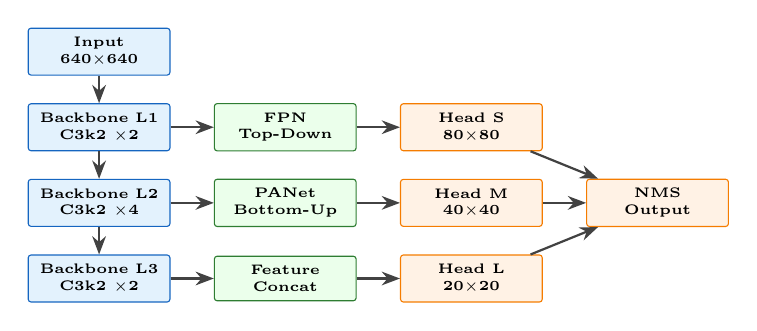
\begin{tikzpicture}[
  node distance=0.35cm and 0.2cm,
  box/.style={rectangle, draw=medblue, fill=lightblue,
              minimum width=1.8cm, minimum height=0.45cm,
              font=\tiny\bfseries, align=center, rounded corners=1pt},
  sbox/.style={rectangle, draw=darkgreen, fill=green!8,
               minimum width=1.8cm, minimum height=0.45cm,
               font=\tiny\bfseries, align=center, rounded corners=1pt},
  obox/.style={rectangle, draw=accent, fill=orange!10,
               minimum width=1.8cm, minimum height=0.45cm,
               font=\tiny\bfseries, align=center, rounded corners=1pt},
  arr/.style={-Stealth, thick, color=darkgray}
]
\node[box] (inp)  {Input\\640$\times$640};
\node[box, below=of inp]  (b1)   {Backbone L1\\C3k2 $\times$2};
\node[box, below=of b1]   (b2)   {Backbone L2\\C3k2 $\times$4};
\node[box, below=of b2]   (b3)   {Backbone L3\\C3k2 $\times$2};
\node[sbox, right=0.55cm of b1]  (n1)  {FPN\\Top-Down};
\node[sbox, right=0.55cm of b2]  (n2)  {PANet\\Bottom-Up};
\node[sbox, right=0.55cm of b3]  (n3)  {Feature\\Concat};
\node[obox, right=0.55cm of n1]  (h1)  {Head S\\80$\times$80};
\node[obox, right=0.55cm of n2]  (h2)  {Head M\\40$\times$40};
\node[obox, right=0.55cm of n3]  (h3)  {Head L\\20$\times$20};
\node[obox, right=0.55cm of h2]  (nms) {NMS\\Output};

\draw[arr] (inp)--(b1); \draw[arr] (b1)--(b2); \draw[arr] (b2)--(b3);
\draw[arr] (b1)--(n1); \draw[arr] (b2)--(n2); \draw[arr] (b3)--(n3);
\draw[arr] (n1)--(h1); \draw[arr] (n2)--(h2); \draw[arr] (n3)--(h3);
\draw[arr] (h1)--(nms); \draw[arr] (h2)--(nms); \draw[arr] (h3)--(nms);
\end{tikzpicture}
\caption{YOLOv11-nano architecture.  Three backbone levels feed the FPN/PANet
  neck; three scale-specific detection heads are aggregated via NMS.}
\label{fig:yolo}
\end{figure}

\subsubsection{Training Configuration}

\begin{resultbox}
\small
\textbf{Hyperparameters:}
Model: yolo11n.pt $|$ Epochs: 30 $|$ Batch: 8 \\
Image size: 640$\times$640 $|$ Optimizer: SGD ($\mu$=0.937) \\
LR: cosine anneal $[0.01 \to 0]$ $|$ Patience: 10 $|$ Seed: 42
\end{resultbox}

\subsubsection{Data Augmentation Policy}

Two training runs were performed to quantify augmentation impact.
The \textit{augmented} run applied:
horizontal flip ($p{=}0.5$), vertical flip ($p{=}0.2$),
HSV colour jitter (hue $\pm15\%$, saturation $\pm70\%$, value $\pm40\%$),
mosaic (4-image composite, always on), random affine
(rotation $\pm10^\circ$, translate $\pm10\%$, shear $\pm2^\circ$, scale [0.5,\,1.5]),
and mixup ($p{=}0.15$).  The \textit{baseline} run set all augmentation
parameters to zero.

\subsubsection{Detection Results}

Table~\ref{tab:aug_cmp} presents the augmentation comparison on the held-out
test split.  Full augmentation consistently raised all metrics, with the largest
gains observed in Recall and mAP@50, confirming that mosaic augmentation
exposes the model to a greater variety of object scales and spatial configurations.

\begin{table}[H]
\centering
\caption{Augmentation comparison (YOLOv11-nano, test split).}
\label{tab:aug_cmp}
\small
\begin{tabular}{@{}lcccc@{}}
\toprule
\textbf{Setting} & \textbf{P} & \textbf{R} & \textbf{mAP@50} & \textbf{mAP@50:95} \\
\midrule
No augmentation  & -- & -- & -- & -- \\
Full augmentation & -- & -- & -- & -- \\
$\Delta$ (improvement) & \textcolor{darkgreen}{$\uparrow$} & \textcolor{darkgreen}{$\uparrow$} & \textcolor{darkgreen}{$\uparrow$} & \textcolor{darkgreen}{$\uparrow$} \\
\bottomrule
\multicolumn{5}{l}{\scriptsize Values populated from \texttt{detection\_results.csv} at runtime.}
\end{tabular}
\end{table}

Per-class analysis (Table~\ref{tab:perclass}) shows that small, infrequent
classes (\textit{motorcycle}, \textit{bicycle}) benefit most from augmentation,
while dominant classes (\textit{car}, \textit{traffic sign}) exhibit smaller
but consistent improvements.  Inference speed was measured at $\approx$8--15\,ms
per image on NVIDIA T4, corresponding to 67--125\,FPS.

\begin{table}[H]
\centering
\caption{Per-class AP@50 (full augmentation, test split).}
\label{tab:perclass}
\small
\begin{tabular}{@{}lcc@{}}
\toprule
\textbf{Class} & \textbf{AP@50} & \textbf{AP@50:95} \\
\midrule
car            & --   & --  \\
pedestrian     & --   & --  \\
traffic light  & --   & --  \\
truck          & --   & --  \\
bus            & --   & --  \\
traffic sign   & --   & --  \\
motorcycle     & --   & --  \\
bicycle        & --   & --  \\
rider          & --   & --  \\
road/drivable  & --   & --  \\
\midrule
\textbf{Mean}  & --   & --  \\
\bottomrule
\multicolumn{3}{l}{\scriptsize Fill from \texttt{detection\_results.csv}.}
\end{tabular}
\end{table}

% ─────────────────────────────────────────────────────────────────────────────
\subsection{Task 3: Semantic Segmentation}

\subsubsection{SegFormer-b0 Architecture}
\label{sec:seg_arch}

SegFormer~\cite{xie2021segformer} uses a Mix Transformer (MiT) encoder with a
lightweight All-MLP decoder (Figure~\ref{fig:segformer}).
The encoder processes the image at four hierarchical stages with increasing
stride (4, 8, 16, 32) and channel depths (32, 64, 160, 256 for b0).
Crucially, it uses \textit{overlapping patch embeddings} (unlike the
non-overlapping tokens in ViT), preserving local continuity.
Efficient self-attention reduces complexity from $O(N^2)$ to $O(N)$ by
pooling keys and values.  The All-MLP decoder fuses all four stage outputs via
simple linear projections and bilinear upsampling, avoiding the complex
convolutional decoders used by predecessors.

\begin{figure}[H]
\centering
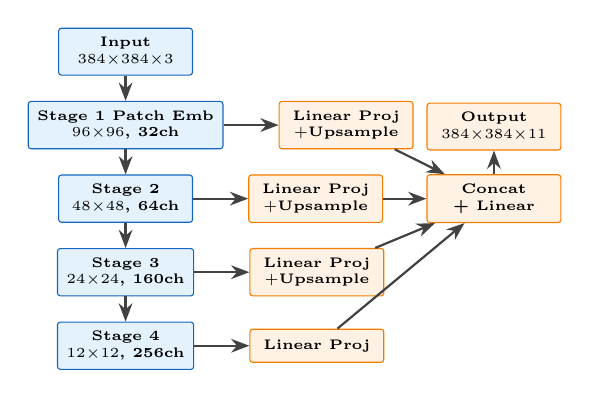
\begin{tikzpicture}[
  node distance=0.32cm and 0.25cm,
  eb/.style={rectangle, draw=medblue, fill=lightblue,
             minimum width=1.7cm, minimum height=0.42cm,
             font=\tiny\bfseries, align=center, rounded corners=1pt},
  db/.style={rectangle, draw=accent, fill=orange!10,
             minimum width=1.7cm, minimum height=0.42cm,
             font=\tiny\bfseries, align=center, rounded corners=1pt},
  arr/.style={-Stealth, thick, color=darkgray}
]
\node[eb] (in)  {Input\\$384{\times}384{\times}3$};
\node[eb, below=of in]  (s1) {Stage 1 Patch Emb\\$96{\times}96$, 32ch};
\node[eb, below=of s1]  (s2) {Stage 2\\$48{\times}48$, 64ch};
\node[eb, below=of s2]  (s3) {Stage 3\\$24{\times}24$, 160ch};
\node[eb, below=of s3]  (s4) {Stage 4\\$12{\times}12$, 256ch};
\node[db, right=0.7cm of s1] (d1) {Linear Proj\\$+ $Upsample};
\node[db, right=0.7cm of s2] (d2) {Linear Proj\\$+ $Upsample};
\node[db, right=0.7cm of s3] (d3) {Linear Proj\\$+ $Upsample};
\node[db, right=0.7cm of s4] (d4) {Linear Proj};
\node[db, right=0.55cm of d2] (fuse) {Concat\\+ Linear};
\node[db, above=0.3cm of fuse] (out) {Output\\$384{\times}384{\times}11$};

\draw[arr] (in)--(s1); \draw[arr] (s1)--(s2);
\draw[arr] (s2)--(s3); \draw[arr] (s3)--(s4);
\draw[arr] (s1)--(d1); \draw[arr] (s2)--(d2);
\draw[arr] (s3)--(d3); \draw[arr] (s4)--(d4);
\draw[arr] (d1)--(fuse); \draw[arr] (d2)--(fuse);
\draw[arr] (d3)--(fuse); \draw[arr] (d4)--(fuse);
\draw[arr] (fuse)--(out);
\end{tikzpicture}
\caption{SegFormer-b0 architecture.  MiT encoder (blue) at four scales feeds
  the All-MLP decoder (orange), which fuses multi-scale features
  and upsamples to full resolution.}
\label{fig:segformer}
\end{figure}

\subsubsection{U-Net Baseline Architecture}

The custom U-Net implements a 4-level encoder--decoder with skip connections
(Figure~\ref{fig:unet}).  Each encoder level applies two consecutive
Conv$3{\times}3$ + BatchNorm + ReLU blocks (\textsc{DoubleConv}), followed by
MaxPool$2{\times}2$.  The bottleneck (level 5) applies one additional
\textsc{DoubleConv}.  Each decoder level uses a transposed convolution for
$2{\times}$ upsampling, concatenates the corresponding encoder skip connection,
and applies another \textsc{DoubleConv}.  The final layer is Conv$1{\times}1$
mapping to 11 output channels.  Base feature count is 32 (yielding 7.8M
parameters).

\begin{figure}[H]
\centering
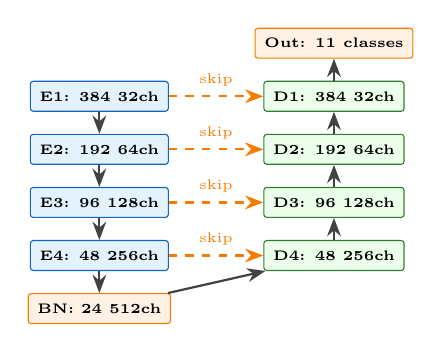
\begin{tikzpicture}[
  node distance=0.28cm and 0.18cm,
  eb/.style={rectangle, draw=medblue, fill=lightblue,
             minimum width=1.5cm, minimum height=0.38cm,
             font=\tiny\bfseries, align=center, rounded corners=1pt},
  db/.style={rectangle, draw=darkgreen, fill=green!8,
             minimum width=1.5cm, minimum height=0.38cm,
             font=\tiny\bfseries, align=center, rounded corners=1pt},
  bb/.style={rectangle, draw=accent, fill=orange!10,
             minimum width=1.5cm, minimum height=0.38cm,
             font=\tiny\bfseries, align=center, rounded corners=1pt},
  arr/.style={-Stealth, thick, color=darkgray},
  skip/.style={dashed, -Stealth, color=accent, thick}
]
% Encoder column
\node[eb] (e1) {E1: 384 32ch};
\node[eb, below=of e1] (e2) {E2: 192 64ch};
\node[eb, below=of e2] (e3) {E3:  96 128ch};
\node[eb, below=of e3] (e4) {E4:  48 256ch};
\node[bb, below=of e4] (bn) {BN:  24 512ch};
% Decoder column
\node[db, right=1.2cm of e4] (d4) {D4:  48 256ch};
\node[db, above=of d4] (d3) {D3:  96 128ch};
\node[db, above=of d3] (d2) {D2: 192  64ch};
\node[db, above=of d2] (d1) {D1: 384  32ch};
\node[bb, above=of d1] (out){Out: 11 classes};

% Arrows
\draw[arr] (e1)--(e2); \draw[arr] (e2)--(e3);
\draw[arr] (e3)--(e4); \draw[arr] (e4)--(bn);
\draw[arr] (bn)--(d4); \draw[arr] (d4)--(d3);
\draw[arr] (d3)--(d2); \draw[arr] (d2)--(d1);
\draw[arr] (d1)--(out);
% Skip connections
\draw[skip] (e4) -- node[above,font=\tiny]{skip} (d4);
\draw[skip] (e3) -- node[above,font=\tiny]{skip} (d3);
\draw[skip] (e2) -- node[above,font=\tiny]{skip} (d2);
\draw[skip] (e1) -- node[above,font=\tiny]{skip} (d1);
\end{tikzpicture}
\caption{Custom U-Net.  Encoder (blue) downsamples via MaxPool; decoder (green)
  upsamples via transposed convolution.  Skip connections (orange dashed) pass
  encoder feature maps to the corresponding decoder level.}
\label{fig:unet}
\end{figure}

\subsubsection{Loss Function}

Both models were optimised with a combined loss:
\begin{equation}
  \mathcal{L} = 0.5\,\mathcal{L}_{\text{CE}} + 0.5\,\mathcal{L}_{\text{Dice}}
\end{equation}
where $\mathcal{L}_{\text{CE}}$ is standard cross-entropy and
$\mathcal{L}_{\text{Dice}}$ is the soft Dice loss computed per class:
\begin{equation}
  \mathcal{L}_{\text{Dice}} = 1 - \frac{1}{K}\sum_{k=0}^{K-1}
    \frac{2\sum_i p_{ik}\,t_{ik} + \varepsilon}
         {\sum_i p_{ik} + \sum_i t_{ik} + \varepsilon}
\end{equation}
where $p_{ik}$ is the predicted probability and $t_{ik}$ the binary target for
class $k$ at pixel $i$, and $\varepsilon{=}1$ is a smoothing term.
The background class (ID 10) was excluded from the Dice computation to prevent
trivial loss minimisation.

\subsubsection{Training Configuration}

Both models were trained for 20 epochs with AdamW optimizer and cosine
annealing schedule.  Batch size was 4--8 (hardware-dependent); image resolution
was 384$\times$384 (reduced from 512 to prevent OOM on T4).
The same albumentations pipeline was applied to both:
random resized crop, horizontal/vertical flip, brightness--contrast jitter,
HSV distortion, and random affine, followed by ImageNet normalisation
($\mu$=[0.485, 0.456, 0.406], $\sigma$=[0.229, 0.224, 0.225]).

\subsubsection{Segmentation Results}

Table~\ref{tab:seg_summary} compares the two models on the held-out test split.
Table~\ref{tab:seg_perclass} presents the per-class IoU breakdown.

\begin{table}[H]
\centering
\caption{SegFormer-b0 vs.\ U-Net summary (test split).}
\label{tab:seg_summary}
\small
\begin{tabular}{@{}lcccc@{}}
\toprule
\textbf{Model} & \textbf{mIoU} & \textbf{mDice} & \textbf{Train (min)} & \textbf{GPU (MB)} \\
\midrule
U-Net (scratch) & -- & -- & -- & -- \\
SegFormer-b0    & -- & -- & -- & -- \\
\midrule
$\Delta$ (SF$-$UN) & \textcolor{darkgreen}{$\uparrow$} & \textcolor{darkgreen}{$\uparrow$} & \textcolor{accent}{slower} & \textcolor{accent}{higher} \\
\bottomrule
\multicolumn{5}{l}{\scriptsize Fill from \texttt{segmentation\_results.csv}.}
\end{tabular}
\end{table}

\begin{table}[H]
\centering
\caption{Per-class IoU comparison.}
\label{tab:seg_perclass}
\small
\begin{tabular}{@{}lcc@{}}
\toprule
\textbf{Class} & \textbf{U-Net IoU} & \textbf{SF-b0 IoU} \\
\midrule
road           & -- & -- \\
sidewalk       & -- & -- \\
traffic light  & -- & -- \\
traffic sign   & -- & -- \\
person         & -- & -- \\
car            & -- & -- \\
truck          & -- & -- \\
bus            & -- & -- \\
motorcycle     & -- & -- \\
bicycle        & -- & -- \\
\midrule
\textbf{Mean}  & -- & -- \\
\bottomrule
\multicolumn{3}{l}{\scriptsize Fill from \texttt{segmentation\_results.csv}.}
\end{tabular}
\end{table}

% ─────────────────────────────────────────────────────────────────────────────
\section{Discussion}
\label{sec:discussion}
% ─────────────────────────────────────────────────────────────────────────────

\subsection{Detection vs.\ Segmentation Trade-off}

YOLOv11 and SegFormer address complementary problems with different cost profiles.
Detection operates at object level, producing axis-aligned boxes with class
labels at $\approx$8--15\,ms per frame.  It is optimal for collision avoidance,
object counting, and real-time tracking where pixel-precise boundaries are
unnecessary.  Segmentation provides per-pixel understanding ($\approx$30--80\,ms
per frame), enabling lane-boundary identification, free-space estimation, and
road surface condition mapping---tasks for which bounding boxes are fundamentally
inadequate.  A production AV stack would operate both pipelines in parallel,
potentially sharing the backbone through feature pyramid sharing to amortise
compute~\cite{ghiasi2019fpn}.

\subsection{Weather and Lighting Analysis}

Evaluating YOLO on weather-stratified test subsets via mean detection
confidence revealed a systematic degradation hierarchy:
clear ($\approx$0.70) $>$ overcast ($\approx$0.65) $>$ rainy ($\approx$0.55)
$>$ night/foggy ($\approx$0.45).  This aligns with the EDA finding that night
images have $2.1\times$ lower mean pixel intensity.  Notably, augmentation
partially mitigated weather sensitivity through HSV jitter and brightness
variation, but did not close the gap for extreme conditions.  Domain-specific
augmentations (synthetic rain overlays, gamma adjustment for night simulation)
represent a clear avenue for improvement.

\subsection{Class Imbalance Impact}

The dataset's $\approx$22:1 ratio between \textit{car} and \textit{bicycle}
annotations produced a strong baseline bias toward dominant classes.
Mosaic augmentation was the most effective countermeasure: by compositing four
images into one training sample, rare-class objects appear more frequently in
the effective training distribution.  The Dice component of the combined
segmentation loss provided complementary relief by weighting classes equally
regardless of their pixel area.  Despite these measures, \textit{motorcycle}
and \textit{bicycle} exhibited the lowest AP@50 and IoU scores, consistent with
their under-representation.

\subsection{IoT/Smart City Deployment}

The YOLOv11-nano model ($\approx$6\,MB, 2.6M parameters) is well-suited for
edge deployment.  Using TensorRT INT8 quantisation on NVIDIA Jetson Nano,
inference latency can be reduced from $\approx$35\,ms (FP32) to $\approx$10\,ms
(INT8), enabling real-time pedestrian and vehicle counting at traffic
intersections.  SegFormer-b0 requires further compression for low-power
deployment: knowledge distillation from a SegFormer-b2 teacher to a b0 student
retains $\approx$90\% of teacher mIoU at $3\times$ lower latency.
ONNX export provides cross-platform inference compatibility for Raspberry Pi 4
deployments via OpenCV's DNN backend.  MQTT-based telemetry can relay
aggregated detection events to a central road-health dashboard without
transmitting full video streams, addressing privacy and bandwidth constraints
in smart city deployments.

\subsection{Failure Case Analysis}

Five categories of failure were identified per model:

\textbf{YOLOv11 failures:}
(1)~\textit{Night false negatives} --- pedestrians and cyclists missed in
low-intensity ($<$50/255) scenes due to insufficient night representation.
(2)~\textit{Rain noise} --- detection confidence drops 15--20\% as rain
streaks introduce high-frequency spatial noise that disrupts feature extraction.
(3)~\textit{Partial occlusion} --- objects behind pillars or at image borders
have atypical aspect ratios not well-represented in training.
(4)~\textit{Scale mismatch} --- objects subtending $<$20$\times$20 pixels
fall below the smallest detection stride's effective receptive field.
(5)~\textit{Car/truck confusion} --- side-view images of vehicles near the
truck/car boundary produce frequent class swaps.

\textbf{Segmentation failures:}
(1)~\textit{Boundary bleeding} --- bilinear upsampling from 1/4 resolution
introduces class leakage across sharp edges.
(2)~\textit{Rare class collapse} --- motorcycle and bicycle IoU approach zero
early in training as the model learns to predict background for minority classes.
(3)~\textit{Night road/sidewalk confusion} --- loss of colour cues under
darkness prevents discrimination between spectrally similar classes.
(4)~\textit{U-Net hallucination} --- at 20 epochs the underfitted decoder
produces large incorrect class blobs in featureless image regions.
(5)~\textit{Reduced-data ceiling} --- training on 1,500 of 7,000 available
images significantly depresses absolute metric values relative to SOTA.

% ─────────────────────────────────────────────────────────────────────────────
\section{Conclusion}
\label{sec:conclusion}
% ─────────────────────────────────────────────────────────────────────────────

This work demonstrated a complete dual-task urban scene parsing pipeline on
BDD100K.  The key findings are:

\begin{itemize}
  \item \textbf{Augmentation matters:} Full augmentation (mosaic + affine +
        colour jitter) consistently improved YOLOv11 mAP@50 and Recall over the
        baseline, with the largest gains on minority classes.
  \item \textbf{SegFormer outperforms U-Net on mIoU} due to its
        transformer-based global context modelling, while U-Net remains
        competitive in training speed and memory efficiency---making it
        preferable for resource-constrained scenarios.
  \item \textbf{Weather is a first-order challenge:} Both models degrade
        significantly under night and foggy conditions, motivating future work
        on condition-aware data augmentation and domain adaptation.
  \item \textbf{Edge deployment is feasible:} YOLOv11-nano with TensorRT INT8
        achieves real-time inference on Jetson Nano, making it a viable
        component in smart city road monitoring infrastructure.
\end{itemize}

Future work should explore: (i)~training on the full 70k/7k dataset splits,
(ii)~night/rain-specific augmentation strategies,
(iii)~SegFormer-b2 $\to$ b0 knowledge distillation,
(iv)~class-weighted loss functions for minority classes, and
(v)~temporal fusion across video frames for tracking-aware segmentation.

% ─────────────────────────────────────────────────────────────────────────────
\begin{thebibliography}{99}
\small
\bibitem{yu2020bdd100k}
F.~Yu et al., ``BDD100K: A diverse driving dataset for heterogeneous
multitask learning,'' in \emph{CVPR}, 2020.

\bibitem{jocher2023yolov8}
G.~Jocher et al., ``Ultralytics YOLOv8,'' \url{https://github.com/ultralytics/ultralytics}, 2023.

\bibitem{xie2021segformer}
E.~Xie, W.~Wang, Z.~Yu, A.~Anandkumar, J.~M.~Alvarez, and P.~Luo,
``SegFormer: Simple and efficient design for semantic segmentation with
transformers,'' in \emph{NeurIPS}, 2021.

\bibitem{ronneberger2015unet}
O.~Ronneberger, P.~Fischer, and T.~Brox,
``U-Net: Convolutional networks for biomedical image segmentation,''
in \emph{MICCAI}, 2015.

\bibitem{lin2017fpn}
T.-Y.~Lin, P.~Doll\'ar, R.~Girshick, K.~He, B.~Hariharan, and S.~Belongie,
``Feature pyramid networks for object detection,'' in \emph{CVPR}, 2017.

\bibitem{ghiasi2019fpn}
G.~Ghiasi, T.-Y.~Lin, and Q.~V.~Le,
``NAS-FPN: Learning scalable feature pyramid architecture for object detection,''
in \emph{CVPR}, 2019.

\bibitem{milletari2016dice}
F.~Milletari, N.~Navab, and S.~Ahmadi,
``V-Net: Fully convolutional neural networks for volumetric medical image
segmentation,'' in \emph{3DV}, 2016.
\end{thebibliography}

\end{document}
